\documentclass[sigconf]{acmart}
\usepackage{subcaption}
\usepackage{hyperref}

%\usepackage{endfloat}
%\renewcommand{\efloatseparator}{\mbox{}} % no new page between figures

\usepackage{booktabs} % For formal tables

\settopmatter{printacmref=false} % Removes citation information below abstract
\renewcommand\footnotetextcopyrightpermission[1]{} % removes footnote with conference information in first column
\pagestyle{plain} % removes running headers

\begin{document}
\title{IoT and Big Data Analytics for Equipment Predictive Health Management (PHM)}
\author{Ashok Reddy Singam}
\orcid{HID337}
\affiliation{%
  \institution{Indiana University}
  \streetaddress{711 N Park Ave}
  \city{Bloomington} 
  \state{Indiana} 
  \postcode{47408}
}
\email{asingam@iu.edu}
\author{Anil Ravi}
\orcid{HID333}
\affiliation{%
  \institution{Indiana University}
  \streetaddress{711 N Park Ave}
  \city{Bloomington} 
  \state{Indiana} 
  \postcode{47408}
}
\email{anilravi@iu.edu}
\begin{abstract}
The predictive health management (PHM) is an enabling discipline consisting of technologies and methods to assess the reliability of a product in its actual life cycle conditions to determine the advent of failure and mitigate system risk. The PHM system will monitor environmental, operational, and performance related characteristics of the product and gathered data analyzed to assess product health and predict remaining life. 

In this application, the industrial rotating equipment such as compressors, vacuum blowers, pumps, and valves etc. are considered to monitor and analyze their operational behavior. The product critical operational parameter data such as vibration, temperature, and load current will be collected from field sensors and analyzed to predict the failure using kNN machine learning classification algorithms. The data will be collected from the field using wireless sensors and stored on the cloud based AWS database server. The product data will be analyzed and made available to all stake holders to take appropriate preventive actions via web/mobile applications.
\end{abstract}
\keywords{i523, HID333, HID337, KNN, IoT, Big Data, Analytics}
\maketitle
\section{Introduction}
The PHM technology can be put within a broader business context by relating it to the Product-Service System (PSS) business model. PSS can be defined as an integrated combination of products and services where the emphasis is put on the \lq sale of use \rq rather than the \lq sale of product \rq. Central to this new business model is a shift from selling a product, and its related spare parts as required, to selling a solution that supports customer needs in the form of a service delivering a fully maintained and useable product \cite{Tonci2009}. As shown in Figure 1, There are several wireless technologies such as 802.11, cellular, and short distance wireless protocols  can be used to collect and send data to the centralized servers.Also, data can be stored in cloud based technologies such as AWS, Microsoft Azure, IBM and Google etc. for processing. 


\begin{figure}
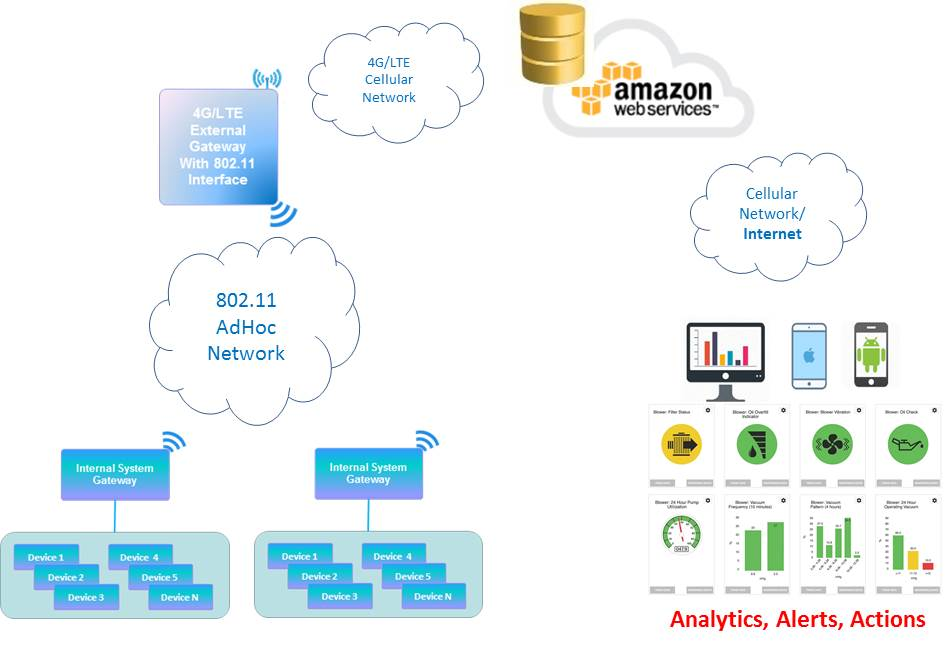
\includegraphics[width=1.0\columnwidth]{images/system_architecture}
\caption{System Architecture} \label{fig:Figure1}
\end{figure}


\textbf{Problem Statement :} in the manufacturing operations, automotive and other process industries rotating equipment such as pumps, valves, compressors, and blowers are commonly used equipment for various purposes. These equipment are severely suffered from wear and tear, bearing degradation, shaft misalignment, corrosion, and other mechanical breakdowns. Due to the limitations of wireless enabled sensors based data acquisition it was very difficult to collect this data in the past. Also, due to real-time nature of the data acquisition, it was a huge challenge to store the data locally and process the information for applying machine learning algorithms. All these technological and infrastructure limitations caused industrial equipment health monitoring had become one of the sector businesses are losing the money due to operation shutdowns and unplanned maintenance etc.

\textbf{Solution Approach :} with the wireless sensors and cloud based server technologies, it has become possible to deploy hundreds of sensors in the manufacturing plant and collect the data and store with minimal costs. Once the data is stored on the servers with high computing power, machine learning algorithms can be used to process the sensor data to predict the equipment failures with reasonable accuracy. This approach has been named as predictive or prognostics health management of the equipment which is widely available in the recent times due to the availability of technological infrastructure.

The PHM generally combines sensing, collecting, storing and analyzing of environmental, operational, and performance related parameters to assess the health of a product and predict remaining useful life. Assessing the health of a product provides information that can be used to meet several critical goals: (1) providing advance warning of failures; (2) minimizing unscheduled maintenance, extending maintenance cycles, and maintaining effectiveness through timely repair actions; (3) reducing the life cycle cost of equipment by decreasing inspection costs, downtime, and inventory; and (4) improving qualification and assisting in the design and logistical support of fielded and future systems \cite{Shunfeng2010}.

The PHM is not a new concept, however, with the advent of sensors, machine learning algorithms, and computing capacity of the servers it has become more prevalent in the recent days. In this application, an attempt has been made to prove the concept of simple PHM implementation and use in real world applications. The application can be re-architected to address more complex products/systems with considerations of scalability, performance, cost and reliability. The limitations of the current application are described in the end of this report.

The parameter monitoring and the analysis of acquired data using prognostic models are fundamental steps for the PHM methods. The sensors are the essential devices used to monitor parameters and obtain long-term accurate information to provide anomaly detection, fault isolation, and rapid failure prediction \cite{Shunfeng2010}.

Firstly, PHM requires monitoring a large number of product parameters to evaluate the health of a product. Depending on the complexity of the monitored product, it is possible to monitor thousands of parameters in the entire life cycle of the product to provide the information required by PHM. These parameters include operational and environmental loads as well as the performance conditions of the product, for example, temperature, vibration, shock, pressure, acoustic levels, strain, stress, voltage, current, humidity levels, contaminant concentration, usage frequency, usage severity, usage time, power, and heat dissipation. In each case, a variety of monitoring features such as magnitude, variation, peak level, and rate of change may be required in order to obtain characteristics of parameters.

In this application, commonly used equipment in industrial and automobile operations such as air compressors, vacuum blowers, and smart valves are considered for analysis. The critical operational parameters of these products will be collected using applicable sensors from the field and fed to a database at regular intervals.

In general design, the frequency of data collection and storage depends on the number of parameters to be analyzed, cost of the system and operational behavior of the equipment. For this application, since products with rotating parts are considered, the critical parameters that would define the health of the equipment are: input or load current, internal ambient temperature, and vibration of the equipment.

The PHM application design process is shown in Figure 2, which describes various steps of the processes involved. For the implementation of this project, the sensor generated data is simulated using SQL scripts due to development time constraints. However, a detailed step-by-step approach is provided if we need to plug-in the sensor modules in to the application.



\begin{figure}
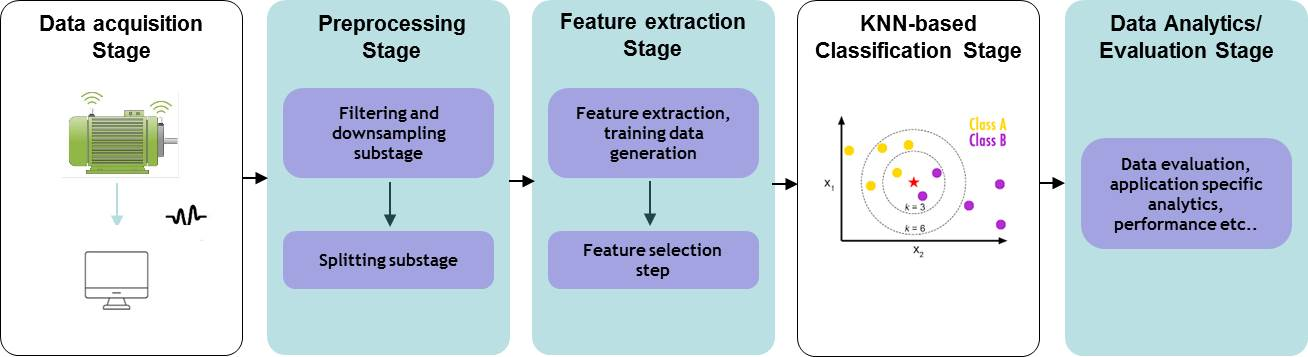
\includegraphics[width=1.0\columnwidth]{images/phm_process_1}
\caption{PHM Design Process} \label{fig:Figure2}
\end{figure}



\textbf{Data Acquisition Stage:} this stage will be the core part of PHM application where vibration data were experimentally obtained from a compressor using triaxial accelerometer to collect transverse, longitudinal and vertical axes vibration signals. For the experimental data collection, ACC301A triaxial accelerometer and National Instruments data acquisition system was used. A total of 8 parameters (1) input current (2) input voltage (3) internal ambient temperature (4) external ambient temperature (5) transverse vibration (6) longitudinal vibration (7) vertical axis vibration and (8) acquisition time were captured at 1 second rate, which generated about 65000 records. This data has been analyzed for identifying the feature classification.

\textbf{Pre Processing stage:} during this stage collected data will be filtered and processed for accuracy in order to adapt them to subsequent feature extraction stage. In this application, all the pre-processing has been done manually to validate the accuracy of the data based on the system conditions. Since spectral analysis of vibration signals are not done ( one of the limitations for this application, captured in the end), the data generated from the compressor is considered as the primary frequency of the equipment (which is isolated from the rest of the attachments).

\textbf{Feature extraction and selection stage:} during this stage domain specific vibration spectral analysis has been performed but only considered time-domain behavior for various system operational conditions such as increased load, modified input voltage, and modified external ambient temperature etc. Based on the response of the machine vibration to various external conditions were noted down. This data is used to identify the following feature vectors.
\begin{itemize}
\item NORMAL OPERATION AT 30 DEG CENTIGRADE
\item OVER CURRENT FAULT OPERATION
\item OVER TEMPERATURE FAULT OPERATION
\item INPUT OVER VOLTAGE FAULT OPERATION
\item ABNORMAL OPERATION AT 30 DEG CENTIGRADE
\item BEARING DEGRADATION OPERATION
\end{itemize}

\textbf{kNN classification stage:} this stage is core part of the PHM application, which will predict the unknown test data to be classified in to a known label based on the training data set using nearest neighbor algorithm.

\textbf{Classifier performance evaluation stage:} this stage will be used to evaluate the classifier accuracy of prediction. In this application, k-fold cross-validation method has been used to perform the evaluation.

The data is generated and made available in Oracle database on AWS cloud to perform analysis. The application developed in this project will consist of the following components:
\begin{itemize}
  \item Sensor Data Generator
  \item Machine Learning Algorithm - kNN
  \item Big Data and IoT
  \item PHM Dashboard
  \item Decision Alert Manager
  \item Installation Script
 \end{itemize}

The following sections will describe the architectural and design aspects of the PHM system implementation in detail.

\section{Prognostics Model Evaluation}
\cite{Saxena2009} The prediction is typically performed only after the \lq\lq health \rq\rq of the component or system deteriorates beyond a certain threshold. In this application, faults and failures are identified in the training data set. The faults identified are: Over current fault, over temperature fault and over voltage fault. If over current fault is occurred, the equipment will tend to draw higher current than nominal values which if continued further several times eventually leads to a permanent failure of the equipment. In this application, when motor bearing starts degrading, the first observation will be over current followed by over temperature conditions.
Often times, that threshold is tripped because a fault occurs. A fault is a state of a component or system that deviates from the normal state such that the integrity of the component is outside of its required specification. A fault does not necessarily imply that the overall system does not operate anymore; however, the damage that characterizes the fault often grows under the influence of operations to a failure. The latter is the state at which the component or system does not meet its desired function anymore. It is the task of prognostics to estimate the time that it takes from the current time to the failed state, conditional on anticipated future usage. This would give operators access to information that has significant implications on system safety or cost of operations. Where safety is impacted, the ability to predict failure allows operators to take action that preserves the assets either through rescue operation or through remedial action that avert failure altogether. Where minimizing cost of operations is the primary objective, predictive information allows operators to avert secondary damage, or to perform maintenance in the most cost-effective fashion. Often times, there is a mix of objectives that need to be optimized together, sometimes weighted by different preferences.

As emphasized above, predictive models evaluation needs to take domain specificities into account. Such specificities cover two aspects: capability of failure prediction and TTF estimation. From the point of view of TTF, it is desirable that a predictive model can generate alerts in a \lq\lq targeted \rq\rq time window prior to a failure. A model that predicts a failure too early leads to non-optimal component use \cite{Yang2014} which will impact the reliability or availability of the system.

\begin{figure}
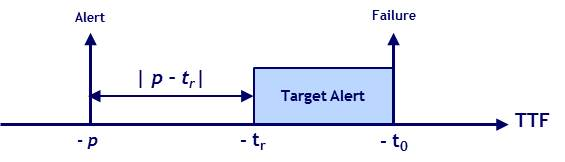
\includegraphics[width=1.0\columnwidth]{images/ttf_1}
\caption{Time relation between alert time and failure time} \label{fig:Figure3}
\end{figure}

As shown in the Figure 3, the time to failure prediction will be estimated based on the classified result data set and alert the stakeholders to take relevant actions. The target alert zone will be identified based on the abnormal behavior of the equipment over the period.

\section{Application Design Analysis}
The PHM application in this project considered to use rotating equipment temperature, load current and vibration data for analyzing and predicting the future operational behavior. 
Vibration signals from rotating components are usually analyzed in the frequency domain, because significant peaks in the signal spectrum appear at frequencies that are related to the rotation frequency of the component. In this application, only time domain parameters with peak vibration magnitudes irrespective of the frequency component. The training data set consists of normal, abnormal, and fault conditions vibration patterns describes the system characteristics from which its status can be estimated.
The PHM application for industrial equipment machine failure detection problem directly correlates to the pattern classification problem. From the vibration data collected, each accelerometer will output values of X, Y, and Z data then using a KNN we can similarly identify which vibration parameter(s) determines problems in our machines, or \lq\lq likely to experience failure.\rq\rq The typical defects or failures that can be detected are: machine imbalance, shaft misalignment, pumps cavitation, structural and rotating looseness, early stage bearing wear, gear teeth problems, and other high-frequency defects.

This application used \lq Sensor Data Gen \rq SQL script module to generate the sensor data and store in Oracle database on AWS. This is the critical module as we have not used the real data collection from the field. However, the sensor hardware and necessary environment to generate the data is identified and experimented to work with. A brief description about the hardware is provided in the end of this report.

The PHM application is designed such that the fundamental concepts can be verified to open a discussion on limitations, performance, scalability, ROI and reliability of the system.

The following sections describe the application design components with necessary implementation details:
\subsection{Sensor Data Generator}
The SQL data generator script is designed to generate training data as well test data for this application with following eleven parameters: Acquisition time, equipment name, part number, serial number, internal ambient temperature, external ambient temperature, input voltage, input current, and vibration data for x, y, and z axes. 
The following database design architecture followed for Sensor Data Gen module:
\begin{itemize}
  \item Sensor Data Generator PL SQL Objects
  \begin{itemize}
  \item Tables
\begin{itemize}
\item SENSOR TRAIN DATA for storing training data
\item SENSOR TEST DATA for storing testing data
\end{itemize}
\item Views
\begin{itemize}
\item SENSOR TRAIN DATA VIEW 
\item SENSOR TEST DATA VIEW
\end{itemize}
\item Packages BIG DATA 503 PRJ PKG
\begin{itemize}
\item Generate Test Set
\item Generate Train Set
\item Delete Data Set
\item Update Test Data Labels
\end{itemize}
\end{itemize}
\end{itemize}

\subsection{Machine Learning Algorithm}
\subsubsection{Classifier evaluation}
Before choosing kNN Model for this project, we performed small experiment to try different models on training data. Below are the results we got. Based on these results we decided to use kNN model.
\begin{itemize}
\item LogisticRregression: 0.963636 (0.044536)
\item KNN: 0.981818 (0.036364)
\item DecisionTreeClassifier: 0.964394 (0.059656)
\item SVM: 0.972727 (0.041660)
\end{itemize}

\begin{figure}
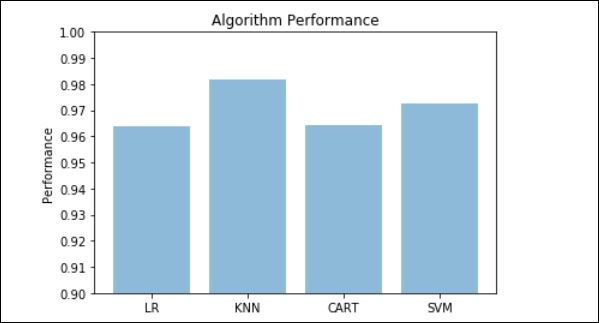
\includegraphics[width=1.0\columnwidth]{images/algperformance}
\caption{Algorithm performance} \label{fig:Figure5}
\end{figure}

\subsubsection{k Nearest Neighbor - kNN}
\cite{Kevin2016} In this application, neighbors-based classification is chosen to classify the unknown instance to the known trained labels. Neighbors-based classification does not attempt to construct a general internal model, but simply stores instances of the training data. Classification is computed from a simple majority vote of the nearest neighbors of each point: a query point is assigned the data class which has the most representatives within the nearest neighbors of the point.
KNN falls in the supervised learning family of algorithms. Informally, this means that we are given a labelled dataset consisting of training observations (x,y) and would like to capture the relationship between x and y. More formally, our goal is to learn a function h:X ->Y so that given an unseen observations x, h(x) can confidently predict the corresponding output y.


In the classification setting, the K-nearest neighbor algorithm essentially boils down to forming a majority vote between the K most similar instances to a given \lq\lq unseen \rq\rq observation. Similarity is defined according to a distance metric between two data points. A popular choice is the Euclidean distance given by:\newline
\[
d(x,x')=\sqrt{(x1-x1\rq)^2+(x2-x2\rq)^2+...+(xn-xn\rq)^2}
\]\newline
But other measures can be more suitable for a given setting and include the Manhattan, Chebyshev and Hamming distance. 
An alternate way of understanding KNN is by thinking about it as calculating a decision boundary (i.e. boundaries for more than 2 classes) which is then used to classify new points.
\subsubsection{K-fold cross-validation}
To estimate the test error in the model, a cross-validation approach followed in which a subset of the training set will be holding out from the fitting process. This subset, called the validation set, can be used to select the appropriate level of flexibility of our algorithm. There are different validation approaches that are used in practice, and we will be exploring one of the more popular ones called \textbf{k-fold cross validation.}
The k-fold cross validation (the k is totally unrelated to K) involves randomly dividing the training set into k groups, or folds, of approximately equal size. The first fold is treated as a validation set, and the method is fit on the remaining \(k-1\) folds. The misclassification rate is then computed on the observations in the held-out fold. This procedure is repeated k times; each time, a different group of observations is treated as a validation set. This process results in k estimates of the test error which are then averaged out. 

In this application, an average k-fold cross validation accuracy of 0.99 achieved, which is explained in the appendix section of the report.

\subsection{Big Data and IoT}
In PHM systems big data is characterized by one or more 3Vs: volume, velocity and variety due to streaming of real-time IoT sensors. Most of the IoT systems present challenges in combinations of velocity and volume. The important feature of the IoT application is that by observing the behavior of \lq\lq many things\rq\rq it will be possible to gain important insights, optimize processes, etc. This requires storing all the events (velocity and volume challenge) to run analytical queries over the stored events and perform analytics (data mining and machine learning) over the data to gain insights.
In general PHM applications, data will be collected through field sensors at specific rate which accounts for large amount of data per day in the order of multi-million records. This data will be stored in any NOSQL or RDBMS based database for storage and processing. Since the big data infrastructure is much reliable and available widely from multiple vendors, it would help to build complex PHM systems with large number of feature vectors for classification. 

In this application, for the demonstration of the concept, the real vibration data from the compressor equipment has been collected via accelerometer sensors. This vibration data has been analyzed in time domain and established the labels based on the compressor design performance parameters. Later, this data analysis is used to design a SQL script for generating training and test data sets. However, the real-time PHM system will have continuous streaming of data coming from hundreds of devices at faster rates (in the order of milliseconds to tens of seconds). This data needs to be captured by reliable and scalable platforms such as AWS IoT or similar and use the machine learning algorithms to classify the unknown data.
\subsection{PHM Dashboard}
Once all the test data set has been classified in to appropriate labels, the prediction of the failure can be performed based on the trending of the equipment behavior over the period. In order to understand the equipment performance insight, following queries will be used on the classified data:
\begin{itemize}
  \item Faults Reported by Equipment Part Number
  \item Faults Reported by Serial Number
  \item Abnormal Behavior by Equipment Part Number
  \item Abnormal Behavior by Serial Number over the period range
\end{itemize}
There can be more application specific information obtained from classified data set to take various decisions. Figure 4 shows various PHM data analytics for this project. Figure 4(a) displays all the serial numbers of equipment 1 with bearing degradation problems. The X axis gives serial numbers while the Y axis gives number of occurrences of bearing degradation for that particular serial number. Similarly Figure 4 (b) and 4 (c) give the details of over temperature and over current faults of various serial numbers.

\begin{figure}

\begin{subfigure}{0.9\linewidth}
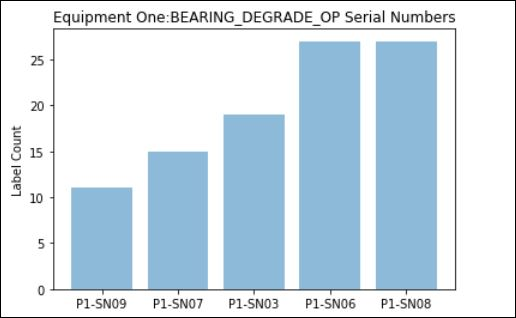
\includegraphics[width=1.0\columnwidth]{images/DEGRADE}
\caption{Bearing Degradation} \label{sfig:sfig4a}
\end{subfigure}

\begin{subfigure}{0.9\linewidth}
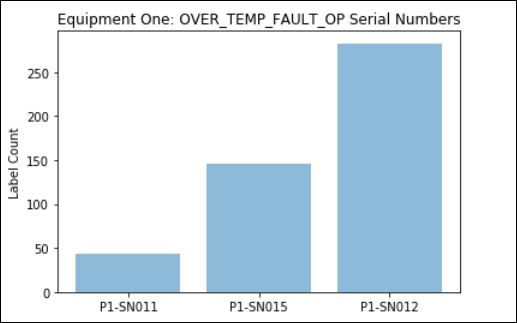
\includegraphics[width=1.0\columnwidth]{images/OVERTEMP}
\caption{Over Temperature Fault} \label{sfig:sfig4b}
\end{subfigure}

\begin{subfigure}{0.9\linewidth}
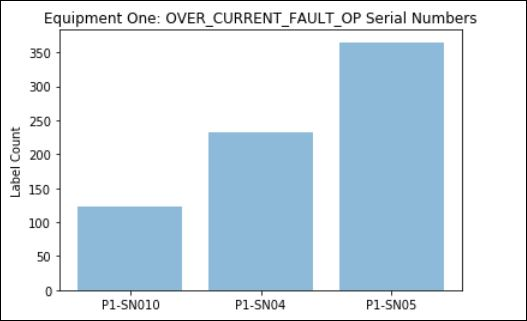
\includegraphics[width=1.0\columnwidth]{images/OVERCURR}
\caption{Over current Fault} \label{sfig:sfig4c}
\end{subfigure}

\caption{PHM Data Analytics} \label{fig:Figure4}
\end{figure}

\subsection{Decision Alert Manager}
Once the results data set has been generated by the prediction algorithm, and then based on the analytics queries, PHM system can send out the alert messages to appropriate stakeholders. The typical messages include the following s minimum:
\begin{itemize}
  \item SN 10002: Faulted X times on over temperature in last Y days, needs maintenance to clean the filter
  \item SN 10005: Consistently indicating bearing degradation from last X days, needs lubrication maintenance
\item SN 10009: Consistently drawing over current from last X days, needs mechanical load maintenance
\end{itemize}

\subsection{Application Script}
All the application specific python modules are captured in a ipynb file which can be run from Jupyter notebook or Github. The location of the file is described in appendix b. This application specific data has been created/generated on AWS cloud database, which will be accessed during the run time by python notebook.
\section{Application Limitations}
The PHM application developed in this project has several limitations. Typically, PHM applications suffer from the prediction accuracy rate which influences the ability to take decisions that will have broader impact on the business operations and financial aspects. However, with the advanced machine learning classifiers and model evaluation methods this can be addressed to achieve reasonable confidence. Following are some of the limitations of this application, which can be addressed and improved in large real-time PHM systems.

\textbf{Data acquisition hardware :} in this application the data is not collected from real-time sensors for voltage, current, temperature and vibration data. There will be inherent accuracy in the raw data generated by SQL script. However, a sample vibration dataset has been collected from the field, which is used as basis to generate the simulated data set.

\textbf{Feature extraction analysis :} the equipment performance parameters of interest need to be down selected from large set of incoming parameter data. 


When analyzing vibration data in the time domain only few parameters are available in quantifying the strength of a vibration profile: amplitude, peak-to-peak value, and RMS.  
The amplitude is valuable for shock events but it does not take into account the time duration and thus the energy in the event. The same is true for peak-to-peak with the added benefit of providing the maximum excursion of the wave, useful when looking at displacement information, specifically clearances. The RMS value is generally the most useful because it is directly related to the energy content of the vibration profile and thus the destructive capability of the vibration.


This requires in-depth domain specific analysis, in this case a detailed mathematical modeling of vibration spectral analysis to precisely select the features and corresponding behavior patterns. Such analytical data should be used for training data feature set. In this application, a primitive approach of time-domain analysis of vibration magnitudes used for determining features. However, in real application these features need to be mathematically analyzed to identify the features that represent the system behavior as close as possible.

\textbf{Model accuracy and scoring :} the kNN algorithm used in this application validated using k-cross fold cross-validation. There are several other model evaluation and scoring methods such as accuracy (or error rate), True Positive Rate (TPR), False Positive Rate (FPR), False Negative Rate (FNR), True Negative Rate (TNR), sensitivity etc. These metrics provide a simple and effective way to measure the performance of a classifier. This application can be further improved by applying more performance measurement methods to increase the effectiveness of the algorithm design.   

\textbf{Scalability :} the application designed in this project is very primitive to understand the basic concepts of PHM and kNN classifier implementation. This application cannot be used for PHM application in business use. To implement real world PHM application, a more comprehensive design needed by considering modularity, service oriented architecture, large number of sensors integration, big data and analytics integration etc.
\section{Conclusion}
In this project, the problem statement around industrial rotating equipment maintenance is described and solution principle to address the same using PHM concept is defined, experimented and results are discussed. Since this application is developed to prove the only concept but not the complete solution a section with limitations and recommendations for real world system development is described. Overall, PHM application with kNN classifier algorithm and cross validation accuracy of 0.99 has been implemented, verified and results are analyzed for business decisions.
\begin{acks}

  The authors would like to thank professor Gregor von Laszewski and his team for providing \textit{LaTex} templates and assistance with the \textit{JabRef} tool to organize references.

\end{acks}

\bibliographystyle{ACM-Reference-Format}
\bibliography{report} 
\newpage
\appendix
\section{Work Breakdown}
\subsection{HID 333:Anil Ravi}
\begin{itemize}
  \item Identified Project topic.
  \item Created architecture of the application.
  \item Ran experimental test to collect vibration data
  \item Extracted and analyzed feature vectors
  \item Studied, designed and reviewed kNN algorithm
  \item Created draft project report
  \item Reviewed the draft project report.
  
\end{itemize}
\subsection{HID 337:Ashok Reddy Singam}
\begin{itemize}
  \item Implemented sensor data generation SQL script.
  \item Implemented kNN algorithm in Python
  \item Implemented k-fold cross validation design
  \item Created data analytics charts
  \item Reviewed the draft project report.
\end{itemize}

\section{Code Reference}
All code, notebooks and files for this project can be found in the githup repository:

\url{https://github.com/bigdata-i523/hid337/blob/master/project/jupyter}


\end{document}
